
\chapter{Discussões}
\label{chapter_discussoes}


% Nesta seção, entraremos em discussões aprofundadas sobre a aplicação da Modelagem Analítica na Avaliação de Desempenho Blockchain como uma abordagem estratégica. Esta metodologia crucial concentra-se na utilização de técnicas de modelagem e análise matemática para avaliar e prever o desempenho da blockchain, abordando aspectos críticos como latência, escalabilidade, segurança e outros parâmetros.

% Abordaremos o papel essencial dos modelos matemáticos na representação do comportamento da rede e a interação de seus componentes. Esses modelos são fundamentais para simular cenários diversos, testar hipóteses e identificar áreas de melhoria ou gargalos na rede blockchain. Destacaremos a relevância dessa abordagem, especialmente em redes públicas de blockchain, onde a competição por recursos e a segurança desempenham papéis cruciais.

% Nossas discussões nesta seção serão guiadas pela aplicação específica da modelagem Markoviana. Através dessa técnica, exploraremos áreas específicas em redes blockchain que podem ser otimizadas para alcançar um desempenho superior do sistema.

% \section{Análise de Consensos por Meio de Cadeias de Markov}

% A modelagem usando Cadeias de Markov para Consensos em DLT (Distributed Ledger Technology) é uma abordagem interessante para entender o comportamento dinâmico desses sistemas descentralizados. Cadeias de Markov são processos estocásticos que evoluem de um estado para outro de acordo com probabilidades de transição, e elas podem ser aplicadas para descrever os estados possíveis de um sistema de consenso em DLT.\cite{bolch2006queueing}

% No contexto de algoritmos de consenso, como Raft e o Tangle para IOTA, a modelagem por Cadeias de Markov pode ser aplicada para analisar e entender o comportamento desses algoritmos em diferentes estados.
% Para a modelagem desses Algoritmos é usado um tipo de processo chamado  Cadeia de Tempo Discreto de Markov (Discrete-Time Markov Chain - DTMC) que  é um modelo estocástico usado para descrever um sistema que evolui em passos discretos no tempo, e cuja evolução entre os estados é regida por probabilidades de transição. Esse modelo é uma extensão das Cadeias de Markov, onde o tempo é contínuo.\cite{ongaro2014search}.

% \subsection{Raft: Um Algoritmo de Consenso}

% O algoritmo de consenso Raft é projetado para ser compreensível, o que facilita a implementação e a depuração. Ele visa resolver os desafios de consenso em sistemas distribuídos, garantindo que todos os nós em um cluster cheguem a um acordo sobre a ordem dos eventos ou transações. O nome "Raft" é uma analogia ao remo em um bote salva-vidas, sugerindo a coordenação e esforço conjunto para avançar na mesma direção.

% O Raft opera com um líder que coordena as atividades e outros seguidores que replicam as instruções do líder. Quando um cliente envia uma transação, ela é encaminhada para o líder, que propaga a operação para os seguidores. A ideia central é garantir que todos os nós no cluster tenham uma visão consistente do estado do sistema.

% O processo de eleição é crucial no Raft. Se o líder falhar, os seguidores iniciam uma eleição para escolher um novo líder. Essa abordagem garante a continuidade da operação mesmo em cenários de falha.

% Além disso, o Raft apresenta um mecanismo de commit que assegura que uma transação seja efetivamente processada em todos os nós antes de ser considerada válida. Isso adiciona uma camada de segurança, evitando que transações se percam ou sejam aplicadas de maneira inconsistente.



% % \textbf{DTMC para Modelagem de Jangada:}
% % Em um cluster Raft, cada nó opera em um dos três estados principais: seguidor, candidato ou líder. Normalmente, apenas um líder está ativo no cluster Raft, e a eleição de líderes ocorre quando necessário. No entanto, situações podem surgir, como divisão de rede, onde dois ou mais líderes são eleitos simultaneamente. Esse cenário pode impactar significativamente o desempenho do sistema, pois os líderes concorrentes podem tomar decisões conflitantes. A modelagem usando Cadeias de Tempo Discreto de Markov (DTMC) é uma abordagem eficaz para analisar e compreender essas dinâmicas complexas no contexto do algoritmo Raft.


%         \begin{figure}[H]
%             \centering
%             \frame{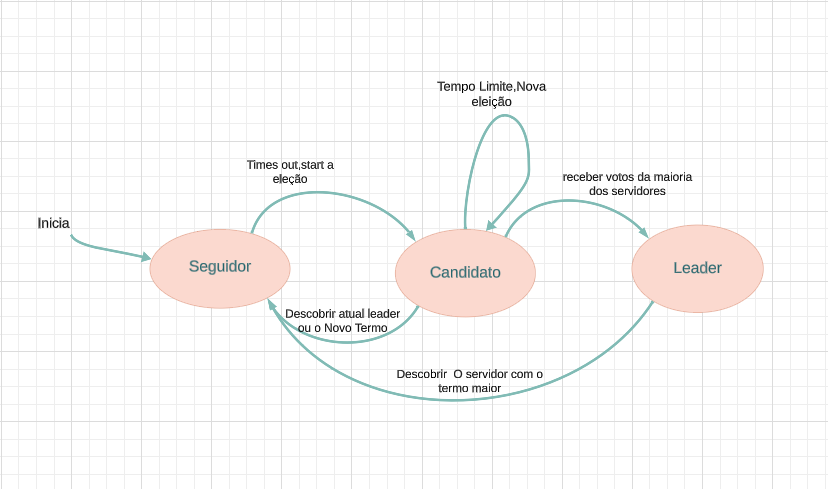
\includegraphics[width=15cm]{6-discussoes/figures/ilustracao_ttransicao.png}}
%             \caption{Ilustração de transição de estados de nó no consenso da Balsa. }
%             \label{Ilustração}
%         \end{figure}

% Para investigar como as características da rede influenciam o desempenho do blockchain, Huang et al. \cite{huang2019performance} desenvolveram um modelo de Cadeia de Markov simplificado para descrever o processo de transição de um nó do estado de seguidor para candidato. Neste contexto, eles analisaram a probabilidade de uma divisão na rede em relação ao tamanho da rede, à taxa de perda de pacotes e ao período de tempo limite para eleições.

% Para a análise, foi definido a probabilidade de perda de pacotes como um valor constante para uma determinada rede, o período de tempo limite para cada rodada de eleição como $\mathbf{E}_t$	, uniformemente iniciado a partir de um intervalo \textbf{[a,b]}, e o intervalo entre dois batimentos cardíacos como . Assim, o número máximo de batimentos cardíacos para um limite de tempo de eleição é  $\bm{\tau}$. Assim, o número máximo de batimentos cardíacos para um limite de tempo de eleição é 
% $K \in \{ K_1, K_2, \ldots, K_r \}$, onde $K_1 = \lfloor a/\tau \rfloor$ e $K_r = \lfloor b/\tau \rfloor$.
% Agora, pode ser definido dois processos estocásticos discretos no tempo: \(g(n)\) como o estágio \(\{1, 2, ..., r\}\) de um nó específico e \(b(n)\) como as etapas restantes (ou seja, número de batimentos cardíacos) para a fase eleitoral antes do tempo limite em um período.

% Assim, o processo de transição de um nó do estado de seguidor para candidato pode ser representado como um processo estocástico bidimensional \(\{ g(n), b(n) \}\), podendo ser transformado em uma Cadeia de Markov Absorvente no espaço de estado \(\{(1, K_1), ..., (1, 0), ..., (i, K_1), ..., (i, 0), ..., (r, K_r), ..., (r, 0)\}\).
% Utilizando as derivações matemáticas apresentadas em \cite{huang2019performance}, é possível obter a probabilidade de uma divisão na rede antes do n-ésimo passo. Este método fornece uma base analítica robusta para entender o impacto das condições de rede na transição de estados dos nós no contexto de blockchain.

% Em resumo, o algoritmo Raft proporciona um meio eficaz e compreensível para alcançar consenso em sistemas distribuídos, contribuindo para a confiabilidade e consistência das operações em um ambiente descentralizado.

% \subsection{IOTA: Um Algoritmo de Consenso Inovador}

% O IOTA se destaca como uma inovação no campo dos algoritmos de consenso, adotando uma abordagem diferente dos modelos tradicionais baseados em blockchain. Em vez de utilizar uma cadeia de blocos, o IOTA emprega uma estrutura chamada Tangle, que é uma espécie de grafo direcionado acíclico.

% A principal característica do Tangle é que ele não possui blocos nem uma estrutura linear de transações. Em vez disso, cada transação se conecta a duas transações anteriores, formando uma rede. Esse design elimina a necessidade de mineradores e permite uma escalabilidade potencialmente ilimitada.

% No Tangle, para realizar uma transação, o usuário deve validar duas transações anteriores. Esse processo de validação é fundamental para manter a segurança e a integridade da rede. À medida que mais transações são realizadas, a rede se torna mais segura e rápida, pois cada nova transação contribui para a validação de outras.
% O IOTA Tangle \cite{guo2020characterizing} é um livro-razão distribuído baseado em DAG projetado para microtransações na IoT. Seu processo de consenso incentiva todos os participantes a contribuir para a manutenção do livro-razão, referenciando duas transações não aprovadas, chamadas dicas, antes de emitir uma nova transação. O Tangle utiliza o algoritmo de caminhada aleatória MCMC para selecionar duas dicas. Todas as transações aprovadas, direta ou indiretamente por esta nova transação, adicionam seu peso cumulativo, conforme demonstrado na Figura 6. À medida que uma transação é aprovada, seu peso cumulativo aumenta gradualmente até atingir um limite predefinido. Finalmente, a transação correspondente é considerada confirmada e registrada permanentemente no livro-razão.

% A ausência de taxas de transação e a eliminação de mineradores tornam o IOTA uma solução atrativa para micropagamentos e Internet das Coisas (IoT), onde eficiência e baixo custo são cruciais. O Tangle é projetado para ser leve e eficiente, tornando-se uma alternativa inovadora em comparação com os modelos tradicionais baseados em blockchain.\cite{guo2020characterizing}

%         \begin{figure}[H]
%             \centering
%             \frame{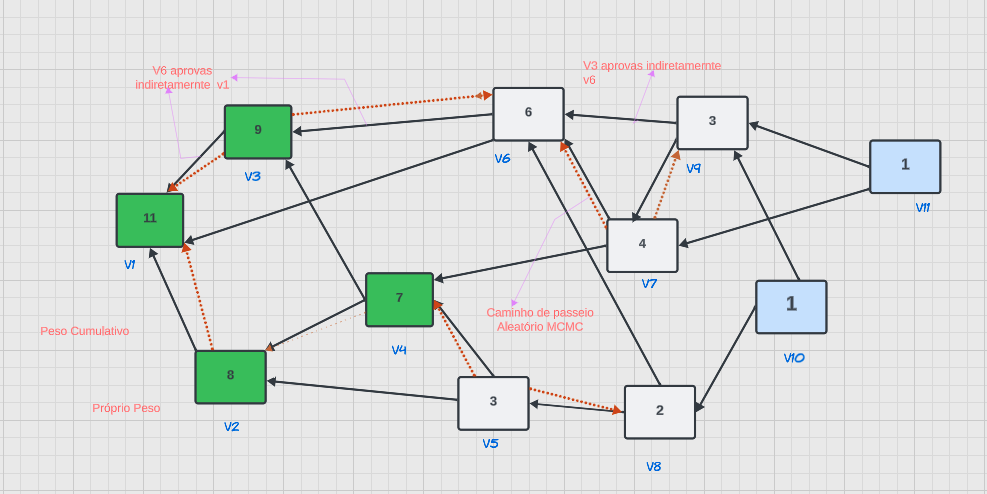
\includegraphics[width=15cm]{6-discussoes/figures/exemplo_IOTA.png}}
%             \caption{exemplo de IOTA. }
%             \label{Exemplo}
%         \end{figure}

% Cao et al. \cite{cao2019impact} propuseram um modelo de cadeia de Markov para analisar o impacto das diferentes taxas de chegada de transações no peso cumulativo e no atraso de confirmação em um sistema de emaranhado. A rede foi categorizada em quatro regimes de carga distintos: alta carga (HR), baixa carga (LR), carga alta a baixa (H2LR) e baixa carga (L2HR)\cite{guo2020characterizing}. O processo de consenso em cada regime foi dividido em dois estágios: revelação e acumulação. O sistema foi modelado como um processo estocástico bidimensional \(S(t) = W(t), L(t)\) em um momento \(t\), onde \(W(t)\) representa o peso cumulativo de uma transação observada e \(L(t)\) é o número total de pontas no emaranhado. O processo de consenso, desde a emissão até a confirmação, foi formulado como um processo Markov e formalizado como um DTMC em intervalos discretos de chegada de transações. A transição de uma etapa da transação observada foi definida como a chegada de uma transação, com a seleção aleatória de duas dicas para referência. Com base neste modelo DTMC, foi possível obter o peso cumulativo esperado e o atraso de confirmação em um determinado momento nos regimes H2LR e L2HR.
 



% Em síntese, o IOTA introduz uma abordagem única e inovadora para o consenso descentralizado por meio do Tangle, proporcionando eficiência, escalabilidade e adequação para casos de uso específicos, como micropagamentos e ambientes de IoT. 




O blockchain, desde sua concepção revolucionária com o advento do Bitcoin em 2008, tem passado por uma notável trajetória de evolução. Nos últimos anos, observamos avanços significativos na tecnologia, impulsionados pela busca incessante por soluções para desafios preexistentes e pela expansão contínua de casos de uso em diversos setores.

Inicialmente concebido como a infraestrutura subjacente para criptomoedas, o blockchain tem ampliado suas fronteiras muito além do escopo financeiro. Uma das transformações mais marcantes é a expansão para contratos inteligentes. Esses protocolos autoexecutáveis não apenas automatizam processos, mas também introduzem uma camada de programabilidade ao blockchain, permitindo uma gama diversificada de aplicações.

O algoritmo de consenso, fundamental para a segurança e integridade do blockchain, também testemunhou mudanças notáveis. A transição do Proof-of-Work (PoW) para alternativas como Proof-of-Stake (PoS) e outras abordagens tem sido debatida intensamente. Essa busca por mecanismos de consenso mais eficientes visa mitigar preocupações ambientais associadas ao alto consumo de energia do PoW, enquanto busca melhorar a escalabilidade das redes.

O blockchain, outrora restrito às criptomoedas, tornou-se uma tecnologia adotada em setores como saúde, logística e governança. Inovações em segurança e privacidade são centrais para essa expansão, proporcionando confiança nas aplicações do blockchain em ambientes críticos.

Contudo, apesar dos avanços, desafios persistem. A escalabilidade, notoriamente, continua sendo uma área de foco. Soluções como camadas secundárias e a exploração de algoritmos de consenso alternativos buscam endereçar essas preocupações, mas o debate sobre a abordagem mais eficaz permanece em curso.

O diálogo em torno do blockchain nos últimos anos não apenas reflete avanços tecnológicos, mas também destaca a importância crescente da colaboração entre setores. Iniciativas de consórcio e padrões interindustriais estão moldando um ecossistema mais coeso, impulsionando a interoperabilidade e facilitando a adoção em larga escala.

Em suma, a evolução do blockchain nos últimos anos é marcada por um constante fluxo de inovações e ajustes. À medida que a tecnologia amadurece, as discussões em torno de seu papel na sociedade e na economia se intensificam. O blockchain, longe de ser uma tecnologia estática, continua a se metamorfosear, prometendo não apenas revolucionar setores específicos, mas também fundamentar a infraestrutura da próxima era digital.